\subsection{Virtual Machine}
\label{sec:vm}

Relay's instruction set is designed as an abstract machine for executing tensor valued
computations. We can realize this abstract machine by either interpreting it or generating
machine code. This is a tried and true approach utilized by existing languages and languages
runtime such as Java, or C\#.

By lowering the full language to an abstract machine we can reduce it to its core operations,
resulting in a small set of operations we can implement. Our implementation uses a virtual
machine design over an ahead of time compiler. In traditional virtual machines the key
reason to perform ahead of time compilation is to reduce dispatch time, and specialize
away dynamic features such as virtual dispatch.

Due to the design of the Relay instruction set, instruction dispatch is a very minimal
part of the total runtime, the runtime is defined by kernel execution time.
A virtual machine allows easier experimentation and modification at the cost of dynamically
dispatching instructions, though nothing in our design prevents ahead of time compilation
of the instruction set, but it provides little value for this reason.

For example if we need to produce ahead of time
compiled code, we either must generate calls into a runtime system (which is dynamic),
only removing instruction dispatch, or statically schedule limiting flexibility and
extensibility.

Furthermore our use of TVM means all kernels are ahead of time compiled meaning the
code which dominates execution time, remember most kernels are quadratic or cubic in
complexity, have efficient implementations.

Our extensions for dynamically sized kernels also utilize TVM code generation, enabling
ahead compilation of kernels which perform a form of polymorphic inline caching for shapes,
playing a similar role to what an ahead of time compiler does in traditional JITs.



\subsection{Tensor Virtual Machine}

Although Relay defines an IR and formal semantics
  it does not provide an efficient execution mechanism for the full language.
In the tradition of definitional interpreters we introduced
  a simple interpreter for Relay which implements its formal semantics, which
  we have separately formalized.
Relay’s interpreter can execute the full language but has notable limitations
  that make it unsuited for production deployments.
It is structured as an inefficient interpreter that performs AST traversal to execute the program.
This approach is conceptually simple but inefficient, as the AST traversal heavily relies on indirection.
For example the initial Relay prototype reused the existing ``graph runtime'', to obtain
  acceptable performance for vision tasks.
The graph runtime can only execute simple control-free,
  DAGs of operations.
We can optimize Relay programs and map a subset of them
  to the graph runtime, but any use of new Relay features
  are unsupported.
By introducing models which make use of new features such
  as control flow, recursion, dynamic shapes, and dynamic allocation,
  we must change how execution works.
There are further challenges in compiling dynamic code, such as dynamic scheduling and allocation,
  fully dynamic tensor shapes, and control flow.
The interpreter offers simple solutions for these, but none is sufficiently compelling or optimized.
The simplicity of the graph runtime provides attractive
  properties such as simple serialization, straightforward
  optimal memory layout, and ease of deployment.

To address these challenges we designed a new Relay
  virtual machine.
The Relay virtual machine balances framework the competing approaches to execution,
  providing a dynamic execution environment which can be extended, instrumented, and integrated with other approaches
  like ahead-of-time compilation via a flexible extension mechanism.
The virtual machine is designed to strike a balance between performance and flexibility
  when deploying and executing Relay programs, without giving up the benefits of TVM.
Virtual machine (VM) design is a well-studied area in programming languages and systems,
  and there have been various virtual machine designs for both full-fledged and embedded programing languages.
Previous language VM designs have been heavily tailored to the execution profile of traditional programs.
Traditional programs manipulate small scalar values
  and consist of a large number of low-level instructions.
The sheer quantity of instructions requires instruction execution
  and dispatch to be extremely efficient.
In the context of machine learning we manipulate primarily tensor values,
  using a (relatively) low number of high level instructions.
ML programs’ cost centers are expensive operator invocations,
  such as GEMM or convolution, over a large input.
Due to the execution profile exhibited by ML programs,
  micro-optimizations present in scalar VMs are dramatically less important.

The Relay virtual machine implement a simple register based VM.

The VM consists of three pieces:
\begin{enumerate}
  \item A tensor instruction set for a tensor virtual machine.
  \item A compiler from Relay to the tensor VM.
  \item An implementation of the virtual machine.
\end{enumerate}

\subsection{ISA}
\begin{itemize}
    \item \verb|ret| Returns a value.
    \item \verb|invoke_packed| Invoke a packed function with the specified arguments.
    \item \verb|alloc_tensor| Allocate a tensor of the given size.
    \item \verb|alloc_datatype| Allocate a datatype with the fields.
    \item \verb|alloc_closure| Allocate a closure.
    \item \verb|get_field| Project a field.
    \item \verb|if| Conditional jump based on the condition register.
    \item \verb|get_tagi| Get the object's tag.
    \item \verb|fatal|
    \item \verb|invoke| Invoke a Relay function.
    \item \verb|invoke_closure| Invoke a Relay closure.
    \item \verb|load_const| Load a constant from the constant pool.
    \item \verb|int_const| Store a constant integer in destination.

\end{itemize}
\subsection{VM Compiler}

In order to execute on the VM we wrote a new compiler which
  can lower Relay directly on to the VM bytecode, and then
  executed.
The compiler performs a set of transformations on the high-level
  Relay program before generating code:
\begin{itemize}
  \item A-Normal Form, converts program in to a limited single-assignment form.
  \item Lambda Lift, converts inline functions into top-level definitions,
        ensuring that capture lists are now explicit.
  \item Inline Primitives, ensures that fused functions are inlined into
        the program to enables simplified code generation.
  \item Inliner, general function inlining.
  \item Constant Pool Layout, traverse program collecting all constant values
        and layout them out in memory.
  \item ADT Tag Allocation, allocate the tag assignment for compilation
        to the VM.
\end{itemize}


\section{System Overview}
\label{sec:Relay-overview}

% \begin{figure}[t]
%   \centering
%   \includegraphics[width=\linewidth]{figs/Relay.pdf}
%   \captionof{figure}{Relay overview. Relay consists of a compiler that handles model with dynamism and a runtime that executes dynamic models in multiple platforms. Both components have multiple modules, which will be introduced in detail in the corresponding sections.}
%   \label{fig:vm}
% \end{figure}

After reviewing systems for dynamic deep learning models, this section gives an overview of Relay, a high-performance and flexible system for compiling and optimizing dynamic models for multiple platforms. In general, the design goals of Relay are:
\begin{enumerate}[leftmargin=*]
    \itemsep 0em
    \item {\bf Supporting dynamic models.} Relay targets models with all types of dynamism, including control flow, dynamic data structures and varied data shapes.
    \item {\bf Being portable and light-weight.} The module that Relay produces should be executable across a number of platforms on the cloud (high-end CPUs and GPUs) and at the edge (low-power CPUs and GPUs). The runtime should be light enough to run on devices with minimal compute power and memory capacity.
    \item {\bf Enabling high performance.} Relay should be performant in the context of dynamism across platforms.
\end{enumerate}

Figure~\ref{fig:vm} shows the system architecture of Relay that we propose to achieve the aforementioned design goals.
It is a system consisting of two major components, namely a compiler and a runtime.
Relay takes a model in the format of mainstream deep learning frameworks, converts it into a unified intermediate representation (\textit{IR}), then optimizes and compiles the IR into an executable that contains both platform-agnostic bytecode and platform-dependent kernel code, and finally loads the executable to execute in the VM-based runtime.
%\yida{The VM high-level description may be moved to the next paragraph, after compiler high-level description.}
%The bytecode is designed to only express the semantics of the IR, e.g. the control-flow and platform-dependent kernel invocation, through dedicated instructions, which contributes a negligible portion of the total execution time, as we will show in~\autoref{sec:eval}.
The bytecode is executed by Relay's runtime interpreter, which is shareable across various platforms.
This design effectively enables us to only maintain one version of the execution logic, but focus more on the performance critical operator kernels.
The kernels are highly-optimized for a specific hardware platform to achieve high performance.
%Kernels optimized for data with different shapes are compiled separately and dispatched accordingly.

To effectively support dynamic models without performance degradation for static models, we introduced various analysis and optimization techniques in Relay's compiler.
First, a set of IR extensions are devised to represent dynamic shapes (\textit{Any} shape) and dynamic allocations for static optimization of dynamic program behaviors (\autoref{sec:compliation:typing}).
Second, shape functions are attached to operators to compute the output shapes dynamically and perform type checking at runtime (\autoref{sec:compilation:shape-func}).
Third, a memory planning optimization is employed to reduce amount of memory consumed (\autoref{sec:compliation:memory}).
Fourth, a heterogeneous device placement mechanism is designed to place IR nodes on ``the-best'' device to reduce expensive cross-device data transferring and synchronization (\autoref{sec:compliation:hetero}).
Finally, the compiler features a code generator that is capable of specializing the code generation of certain likely shapes (\autoref{sec:compliation:codegen}). Once the executable with dynamic behavior is compiled, the VM-based runtime can load and interpret it with intelligent dynamic kernel dispatching (\autoref{sec:runtime}). We detail the design and implementation of each of these features in the followed sections.

\section{Virtual Machine}
\label{sec:runtime}
The conventional runtime of existing deep learning compilers which naively executes a model node by node in topological order does not work for executing the compiled modules of dynamic models. A more intelligent and powerful execute engine is required to handle the control flow execution logic, and dispatch different kernels accordingly. In order to achieve these goals and be portable to different platforms, we design and implement a virtual machine (VM)-based runtime.

In Relay, we compile a dynamic model into a {\em VM executable} that contains platform-independent bytecode and platform-dependent kernel code, which can be later loaded and executed.
The bytecode consists of a series of instructions that predicate the order of kernel invocation and control flow execution logic.
This design compliments conventional runtime's capability for executing highly optimized kernels but not directly handling orchestration between kernels.
%The VM compiler lowers dynamic models to VM instructions, while kernels are lowered to native code via our modified version of TVM.

\subsection{VM ISA}

%The implementation of the VM compiler is straightforward, with the interesting design decisions found in our instruction set's design.
The design of the VM instruction set is motivated by the simple observation that kernel execution dominates neural network execution time. If we treat kernel invocation as a single instruction, the cost of surrounding instructions is negligible in the total execution.

As a result, our design is quite different from traditional language virtual machines, which contain many instructions that perform little work, leading to a profile where the cost of each instruction executed matters.
Our ISA is composed of CISC-style instructions in which each instruction corresponds to a primitive IR expression on tensors, such as allocation and kernel invocation, which in turn may correspond to executing multiple ``low-level'' operations. For example, \texttt{LoadConst idx, \$reg} is capable of multiple addressing modes as it first reads the index \texttt{idx} and then loads the data from a constant pool to the destination register \texttt{\$reg}.
A complete list of instruction set can be found in the appendices.
We naturally select a register-based virtual machine design~\citep{davis2003case} for compact a bytecode, which is easy for users to read and modify. We provide the abstraction of an infinite set of virtual registers as it significantly simplifies optimizations and allocation (similar to SSA) and minimizes conceptual barriers to rapid prototyping and modification.

Instructions are represented using a traditional tagged union containing the op-code and the data payload. This representation enables both efficient serialization and instruction decoding and dispatch. Relay uses variable-length instruction format due to the inclusion of variable sized operands such as data shapes in the instructions.

\begin{comment}
\begin{table*}[t]
\centering
\small
\input{figs/table_isa}
\caption{The opcode and the description of the Relay instruction set \label{tab:isa}}
\end{table*}
\end{comment}

% This design has the following benefits. First, both CISC instructions and variable length encoding contribute to better code density. This is a significant advantage for edge devices that only have limited resources. Second, allowing multiple addressing modes to execute a single instruction can reduce the amount of data fetched from cache hierarchy and main memory. It may also lead to better spatial locality as the data (e.g. the tensor value) may remain in the cache. Third, a variable-length instruction encoding paves the way for extending extra information to instructions, e.g. debugging and even branch prediction. Last but not least, the instruction designed in Relay effectively separates hardware-dependent kernels from model control logic. The Relay bytecode is hardware-independent which eases bytecode serialization, and can be paired with hardware-dependent kernels being invoked by the \texttt{InvokePacked} instruction.

\subsection{Interpreter}

After we have generated a VM executable,
%\yida{we never define what is a VM executable}
we can create an interpreter by loading the executable. When execution begins, the interpreter runs a dispatch loop which checks the op-code and executes the appropriate logic, then repeats. As our instructions are coarse-grained (i.e. they can be viewed as super-instructions), the number of branches generated by the dispatch-loop is lower than traditional programming language VMs, adding negligible overhead compared to ahead of time compilation.

VM uses a tagged object representation reminiscent of those used by programming languages such as Haskell, and OCaml. The tagged object representation smoothly integrates with various data structures, including tensors, algebraic data types, and closures. Due to the specialized object representation, VM instructions only need to interact with the coarse-grained data (i.e. tensors) requiring infrequent memory allocation in chunks.

In sum, the interpreter handles instructions in the following categories.
%\yida{somewhat mention interpreter in the above two paragraphs, otherwise it feels disconnected}

\begin{itemize}[leftmargin=*]
    \item Register-to-Register Operations. Register-to-Register operations, e.g. \texttt{Move}, transfers data between different offset of the register file. Objects are reference counted, make use of copy-on-write and passed by reference ensuring register operations are cheap even if the size of underlying container is large.

    \item Memory Operations. Memory operations can allocate space for tensors, load constant tensors, and so on. Due the design of our constant pool, weights (which are constant during inference) can remain in-memory with no specialized support they can be referenced by the\texttt{LoadConst} instruction.

    \item Call Operations. Call operations are the most frequently executed instructions. The ISA
    has specialized call instructions for invoking a global function, a kernel primitive, closure, copying data across devices, reshaping runtime tensors, and calculating the shape of tensors. Kernel primitives are ahead-of-time compiled through and can leverage both compiler-generated kernels and the third-party libraries.
    %\yida{Should we briefly mention how to decide which kernels (in the context of multiple kernels) to invoke? I don't mean whether to invoke compiler-generated kernels or third-party libraries.}

    \item Control Flow Operations. Unconditional jump instructions, e.g. \texttt{ret}, are used by both static and dynamic models to jump to a specific program point. Only dynamic models need conditional control operations to determine the direction of branching. The interpreter updates the PC using the offset from either the true branch or false branch based on the conditional value.
\end{itemize}

\begin{comment}
\lstset { %
    language=C++,
    basicstyle=\ttfamily\footnotesize,% basic font setting
    keywordstyle=\bfseries\color{green!40!black},
    commentstyle=\itshape\color{purple!40!black},
    stringstyle=\color{orange},
}
\begin{figure}[htbp]
\centering
\begin{lstlisting}
void RunLoop() {
  this->pc = 0;
  Index frame_start = frames.size();
  while (true) {
  main_loop:
    auto const& instr = this->code[this->pc];
    switch (instr.op) {
      case Opcode::LoadConst: {
        auto constant_obj = constants[instr.kidx];
        // ...
        RegWrite(instr.dst, const_pool_[instr.kidx]);
        pc++;
        goto main_loop;
      }
      case Opcode::Invoke: {
        // Prepare args and then invoke.
        InvokeGlobal(functions[instr.func_idx], args);
        frames.back().caller_ret_reg = instr.dst;
        goto main_loop;
      }
      case Opcode::InvokePacked: {
        // Invoke primitive functions
        const auto& func = packed_funcs[instr.pidx];
        const auto& arity = instr.arity;
        // Read args from the register file.
        InvokePacked(instr.pidx, func, arity,
                     instr.osize, args);
        // Write outputs to the register file.
        pc++;
        goto main_loop;
      }
      // Other opcodes are omitted
    }
  }
}
\end{lstlisting}
\caption{Relay bytecode interpreter.}
\label{fig:interpreter}
\end{figure}
\end{comment}

\subsection{Discussion}

%\haichen{compare against AOT. discuss other use cases for vm, e.g., resource isolation, security, integration into a larger system}

%The VM can be seen as the realization of a tensor abstraction machine, which corresponds to high-level tensor operations such as allocating a tensor, invoking an operation like conv2d, or performing a device copy.
An alternative solution to the VM could be ahead of time compilation from our abstract machine into machine code.
But due to the granularity of the operations, dispatch time makes up a very small portion of the execution time. More importantly, the VM provides flexibility traditionally attributed to virtual machines and a clear compiler/runtime split.
We see the potential of VM to be integrated as a runtime module into a larger system.
For example, VM can provide resource isolation where multiple inference instances share the same hardware in the cloud. Furthermore, a Quality of Service (QoS)-aware system, e.g., \citep{kang2018hotmobile, Yachir2009rsj}, could leverage VM to pause the current model execution for a higher priority or time-critical model. Last, because of the simplicity of the VM design, one can verify the implementation of VM for security and privacy purposes.

%Our VM is designed to execute the dynamic models by removing the limitations of the existing runtimes which only support statically shaped programs.
%\yida{Mention the bytecode+kernel design. Also mention other potential use case of VM, like isolation?}

%\subsection{Kernel dispatcher}
%Op fusion across control flow, e.g., pushing ops into if/else branch for more fusion.

% we probably want to talk about this in the instruction set or memory planning. No need to have a separate paragraph here.
%The design of Relay focuses on the simplicity without sacrificing performance. In order to accomplish this, we design a tensor VM rather than a scalar VM. In the tensor VM setting, we optimize for cheap ``allocation'' of objects (by trying to avoid real allocation), reuse of static fragments, and the ability to support dynamic shape (i.e jagged tensors). \autoref{fig:vm} depicts the overview design of VM. It essentially contains a compiler and a runtime system. The compiler compiles a Relay program into both hardware dependent and hardware independent modules/libraries. The hardware independent code consists of low-level bytecode that is specifically designed for efficient execution of VM. The hardware dependent code is composed of coarse-grain operators registered in the TVM operator inventory (TOPI). The runtime system takes charge of the execution of generated bytecode, i.e. dispatching the instructions and managing the stack frame and registers. We will detail the design of the VM in the following sections.

%\zhicomment{@haichen,  Do you still need push and pop? I think we probably don't need them now, instead we use \textit{Move} to manage stack. Am I right?}
%\textit{stack-based} and \textit{register-based} virtual machines are the two major types of VM in programming languages. Stack-based VM aims at simplicity, using \textit{push} and \textit{pop} instructions to maintain a unified stack. However, it complicates tasks such as dataflow analysis and enforces certain orders in the execution. Instead, register-based VM design manages registers to designate the operands and results rather than the stack. This type of VM simplifies the calling convention as values are carried by registers. But it may bring some cost in terms of code size as it needs to decode instructions to fetch the values at specific positions. As aforementioned that our VM mainly targets tensor-level instructions instead of low-level machine instructions. The code size is thus generally small. Furthermore, we would emphasize the convenience of optimizations, such as liveness analysis and memory allocation in the model inference scenario. Therefore, the register-based VM provides more benefits which meets our selection.

\section{Evaluation}
\label{sec:eval}

This section evaluates the performance of Relay on dynamic models against existing state-of-the-art solutions, as well as discussing the role of the optimizations performed by Relay. Specifically, the section seeks to answer the following questions:
\begin{enumerate}
    \item What is the overall performance of Relay for dynamic models when compared against state-of-the-art alternatives on various hardware platforms?
    %\item How much overhead does Relay introduce for static models on top of the state-of-the-art solutions?
    \item How much overhead does Relay VM introduce for handling dynamism at runtime?
    \item How effective are the proposed optimization techniques, such as memory planning and symbolic codegen?
\end{enumerate}

%\yida{Evaluate the execution time of the bytecode as a portion of the total execution time, to show that VM overhead is negligible}
%\note{End-to-end: BERT, LSTM, Tree-LSTM on Intel CPU, ARM CPU, NVidia GPU; Relay-runtime vs. graph runtime. Optimization implication: Kernel dispatch or not; memory planning or not; number of dispatched kernels.}
\subsection{Experiment setup}
\label{sec:eval:setup}

All experiments were conducted on Amazon EC2 instances. We evaluated Relay on three hardware platforms: Intel Skylake CPUs (c5.9xlarge, 18 physical cores, hereinafter called {\em Intel CPU}), Nvidia Tesla T4 GPUs (g4dn.4xlarge, 1 card, 2,560 CUDA cores, hereinafter called {\em Nvidia GPU}), and ARM Cortex A72 (a1.4xlarge, 16 physical cores, hereinafter called {\em ARM CPU}). Although all tests are done on the cloud, our results of ARM CPU are portable to the edge devices, e.g. Raspberry Pi, due to the same architecture. %All cores have uniform memory access.

To study the efficiency of Relay in handling dynamic models, we compared it with mainstream deep learning frameworks, including TensorFlow (v1.15), MXNet (v1.6), PyTorch (v1.5) \footnotemark, as well as dynamic-specific systems TensorFlow Fold based on TensorFlow v1.0.
\footnotetext{We use PyTorch v1.4 on ARM CPU because PyTorch v1.5 fails to build on ARM instance.}
%For TensorFlow Fold, its execution latency would include the compilation time (\zhicomment{@haichen, we probably need a bit argument here for why compile time is included.}).
We were unable to compare Relay with Cavs~\citep{xu2018cavs}, JANUS~\citep{jeong2019janus}, or Jeong et al.\citep{jeong2018improving} as none of them is open-source. No public deep learning compiler has claimed support for dynamic models.
%For static models, TVM~\citep{tvm_osdi18} was selected as the baseline to investigate the cost of Relay since it represents the state-of-the-art performance for static models on CPUs~\citep{liu2019optimizing}.

Three popular models that represent different classes of dynamism were chosen in this experiment, viz. LSTM~\citep{lstm} (dynamic control flow), Tree-LSTM~\citep{tree_lstm} (dynamic data structure), and BERT~\citep{devlin2018bert} (dynamic data shape).
The input size / hidden size used in the LSTM and Tree-LSTM model are 300/512 and 300/150, respectively.
%while we use input size 300 and hidden size 150 in the Tree-LSTM model.
We used BERT base implementation.
For LSTM and BERT, we used Microsoft Research's Paraphrase Corpus (MRPC)~\citep{dolan2005microsoft} with variable input lengths as our input dataset. For Tree-LSTM, we used the Stanford Sentiment Treebank (SST)~\citep{socher2013recursive} with various tree structures as the input dataset.
%\note{missing model size, e.g. LSTM number of layers, length, BERT size}
%For the measurement of the overhead on static models, we completed model inference for ResNet~\citep{he2016deep}, MobileNet~\citep{howard2017mobilenets}, VGG~\citep{simonyan2014very}, and SqueezeNet~\citep{iandola2016squeezenet} on the ImageNet dataset~\citep{deng2009imagenet}. Only one input is needed to feed to the system each time for the task of model inference.

\subsection{Overall performance}
\label{sec:eval:overall}
We compare the overall performance of Relay against baselines for each dynamic models. Relay successfully accomplished inference for all models on all platforms. However, not all baseline systems could perform inference for these models. For instance, TensorFlow Fold was not designed to process LSTM and BERT hence no result was obtainable, and Tree-LSTM only runs on PyTorch and TensorFlow Fold as other frameworks cannot handle dynamic data structures. Finally the model inference of Tree-LSTM on Nvidia GPU was omitted as it's hard to saturate GPU compute capability due to too many control flows and its model size, making GPUs less favorable deployment targets.
% typical use cases.

The baseline systems all make use of third-party kernel libraries to achieve high-performance by leveraging the heavily hand-optimized operators. We observe that dynamic models are often well-optimized on a single platform but perform poorly in other frameworks or on other targets. However, Relay has the ability to select either the self-compiled kernels or the ones provided by third-party library based on which one maximizes performance. It uses dynamic dispatch logic to invoke the selected kernels using platform-independent bytecode at runtime. This enables Relay to deliver portable and consistent results as many compiler optimizations are platform agnostic.
%, and Relay has the freedom to choose whatever implementation that produces better performance.

First, the latency results of Relay, MXNet, PyTorch, and TensorFlow on LSTM are shown in \autoref{tab:lstm}. Relay consistently outperforms the baseline on both 1- and 2-layer cases. For example, it reduces the latency of 1-layer LSTM model inference by $\fpeval{round(79.3 / 47.8, 1)}\times$, $\fpeval{round(212.9 / 47.8, 1)}\times$, and $\fpeval{round(301.4 / 47.8, 1)}\times$ over PyTorch, MXNet, and TensorFlow on Intel CPU,
and $\fpeval{round(110.3/93.0, 1)}\times$, $\fpeval{round(135.7/93.0, 1)}\times$, $\fpeval{round(304.7/93.0, 1)}\times$ on Nvidia GPU, respectively.
%On Nvidia GPU, Relay reduces the latency by  over PyTorch, MXNet, and TensorFlow on Nvidia GPU, respectively.
On ARM CPU, Relay decreases the latency numbers even more remarkably, i.e. $\fpeval{round(1729.5 / 182.2, 1)}\times$ over PyTorch, $\fpeval{round(3695.9 / 182.2, 1)}\times$ over MXNet, and $\fpeval{round(978.3 / 182.2, 1)}\times$ over TensorFlow, respectively.
The similar trend applies to 2-layer case of the LSTM model.
We observe that latency on Nvidia GPU is higher than Intel CPU. This is because the size of LSTM model is relative small so that it cannot fully utilize the massive parallelism in the GPU.
The significant performance improvement is due to Relay encoding the control flow into platform-independent instructions that have minimal overhead while deep learning frameworks use control flow specific primitives to process the sequence, which introduces a large performance penalty.

\begin{table}[t]
\centering
\small
\begin{tabular}{p{0.9cm}|ccc|ccc}
\toprule
Unit: & \multicolumn{3}{c|}{1 layer} & \multicolumn{3}{c}{2 layers} \\
$\mu$s/token & Intel & NV & ARM & Intel & NV & ARM \\ \midrule
Relay & \bf{47.8} & \bf{93.0} & \bf{182.2} & \bf{97.2} & \bf{150.9} & \bf{686.4} \\
PT & 79.3 & 110.3 & 1729.5 & 158.1 & 214.6 & 3378.1 \\
MX  & 212.9 & 135.7 & 3695.9 & 401.7 & 223.8 & 7768.0 \\
TF & 301.4 & 304.7 & 978.3 & 687.3 & 406.9 & 2192.8 \\
\bottomrule
\end{tabular}
\caption{LSTM model inference latency of Relay, PyTorch (PT), MXNet (MX), and TensorFlow (TF) on Intel CPU, Nvidia (NV) GPU, and ARM CPU.}
\label{tab:lstm}
\end{table}

Next, we inspect the performance of model inference on Tree-LSTM as exhibited in \autoref{tab:treelstm} by comparing Relay with PyTorch and TensorFlow Fold. The table shows that Relay runs substantially faster than the baselines. On PyTorch, the performance speedups are $\fpeval{round(701.1/40.3, 1)}\times$ on Intel CPU and $\fpeval{round(1711.1/86.3, 1)}\times$ on ARM CPU as PyTorch uses Python to handle the tree data structure. TensorFlow Fold is $\fpeval{round(209.9/40.3, 1)}\times$ slower than Relay on Intel CPU because it has to re-compile upon every input.

\begin{table}[t]
\centering
\begin{tabular}{l|ll}
\toprule
Unit: $\mu$s/token        & Intel     & ARM \\ \midrule
Relay  & \bf{40.3}  & \bf{86.3}  \\
PyTorch & 701.6 & 1717.1  \\
TF Fold & 209.9 & --  \\
\bottomrule
\end{tabular}
\caption{Tree-LSTM model inference latency on Intel CPU and ARM CPU. TensorFlow Fold was not built successfully on ARM CPU.}
\label{tab:treelstm}
\end{table}

Third, \autoref{tab:bert} summarizes the performance of BERT for Relay, MXNet, and TensorFlow. The results indicate that Relay outstrips the baselines for all frameworks on all platforms in the experiment. The reduction in latency compared to the best framework on each platform is $\fpeval{round(455.8/307, 1)}\times$, $\fpeval{round(2995.4/2862.6, 2)}\times$, and $\fpeval{round(125.2/95.2, 1)}\times$ on Intel CPU, ARM CPU, and Nvidia GPU, respectively.
%Surprisingly, Relay is $\fpeval{round(455.8/307, 1)}\times$ faster than MXNet on Intel CPU even the latter was known to be heavily optimized on this platform~\footnote{\url{https://medium.com/apache-mxnet/optimization-for-bert-inference-performance-on-cpu-3bb2413d376c}}.
The reasons are two-fold: (a) similar to frameworks, Relay is also able to use the well-tuned third-party libraries on Intel CPU (MKL) and Nvidia GPU (cuDNN). (b) Relay can further enjoy the benefit of powerful operator fusion brought by the deep learning compiler. One can observe that we obtained more speedups on the ARM CPU for PyTorch and MXNet as the third-party libraries performed less favorable. However, Relay is only slightly faster than TensorFlow on the ARM CPU. This is because the dense operators (contributing to more than 90\% of the overall latency in Bert) on the ARM CPU was not well optimized by the underlying compiler. Therefore, the performance of the combination of operators it selected is on par with the ones used by TensorFlow.

In sum, the evaluation results demonstrate that Relay produces more portable performance for all dynamic models on different platforms. Instead, the performance of frameworks is more platform dependent and varies from model to model.

\begin{table}[t]
\centering
\begin{tabular}{l|lll}
\toprule
Unit: $\mu$s/token    & Intel  &   Nvidia       &  ARM     \\ \midrule
Relay     & \bf{307.0} & \bf{95.2} & \bf{2862.6} \\
PyTorch & 479.5 & 220.4 & 11851.2 \\
MXNet      & 455.8 & 152.9 & 8628.0   \\
TensorFlow & 768.7 & 125.2 & 2995.4 \\
\bottomrule
\end{tabular}
\caption{BERT model inference latency on Intel CPU, Nvidia GPU, and ARM CPU.}
\label{tab:bert}
\end{table}

% \begin{figure}[t]
%     \centering
%     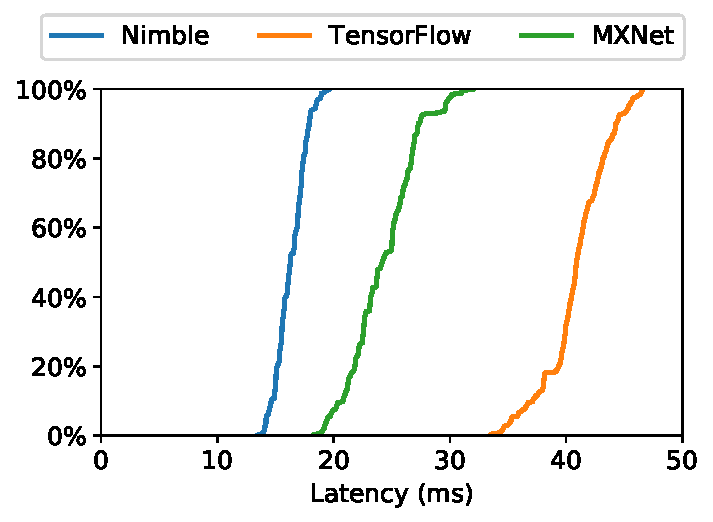
\includegraphics[height=5cm]{figs/bert_cdf_c5.pdf}
%     \caption{BERT latency CDF on Intel CPU.}
%     \label{fig:bert-cdf}
% \end{figure}

%\subsection{Optimization implications}
%\label{sec:eval:opt}
%\subsubsection{Memory planning}

%\subsubsection{Dynamic kernel dispatch}
\subsection{Microbenchmark}

% \begin{table}[t]
%     \centering
%     \begin{tabular}{c|cc|cc}
%         \toprule
%         \multirow{2}{*}{Device} & TVM & Relay  & kernel & others  \\
%         & lat. (ms) & lat. (ms) & lat. (ms) &  (ms) \\ %&  (\%) \\
%         \midrule
%         Intel  & 19.38 & 24.32 & 21.06 & 3.26 \\% & 13.4\%
%         ARM & 223.50 & 237.41 & 228.59 & 8.82 \\%& 3.72\% \\
%         Nvidia & 5.58 & 5.86 & 5.60 & 0.26 \\%& 4.44\% \\
%         \bottomrule
%     \end{tabular}
%     \caption{BERT model latency (sequence length 128) using TVM and Relay on different hardware.
%     {\it kernel latency} shows the latency of kernel invocation in Relay, and {\it others} shows the extra latency introduced by other instructions.
%     }
%     \label{tab:overhead}
%     \vspace{-1em}
% \end{table}

% \hide{
% \begin{figure}[t]
%     \centering
%     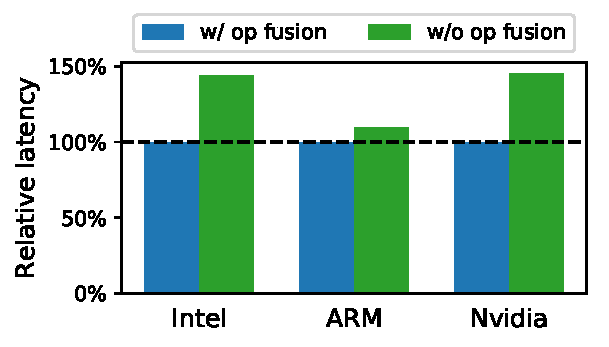
\includegraphics[height=3.5cm]{figs/op_fusion.pdf}
%     \caption{Relative latency comparison between Relay with and without operator fusion for BERT model with sequence length 128.}
%     \label{fig:fusion}
% \vspace{-1em}
% \end{figure}
% }

\begin{figure}[t]
    \centering
    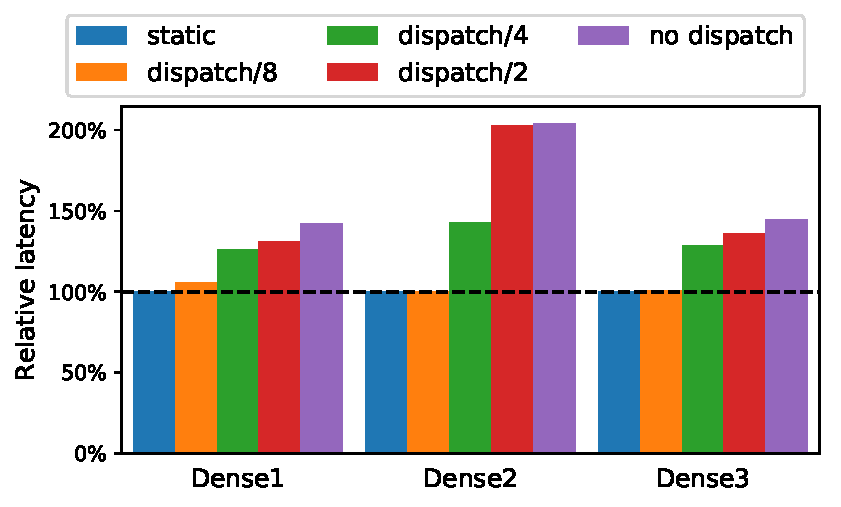
\includegraphics[height=4.5cm]{figs/sym_codegen.pdf}
    \caption{Relative latency comparison between symbolic codegen and static codegen of 3 dense operators on ARM CPU. The latency of kernel compiled with static shapes is used as the baseline. ``dispatch/$k$'' indicates that we generate $k$ symbolic kernels to be dispatched at runtime. ``no dispatch'' means that only one symbolic kernel is generated and therefore no dispatching is needed. %\protect\yida{The labels of x-axis, can we make them Dense 1, Dense 2 and Dense 3? L1, L2, L3 are like cache level to me at the first glance}
    }
    \label{fig:sym-codegen}
\end{figure}

This section analyzes the performance gain of Relay by using BERT as the microbenchmark. Three studies will be conducted to examine (a) the overhead introduced by the VM, %(b) the effectiveness of operator fusion\yida{Can we somehow relate this to any proposed techniques? For example, op fusion is enabled by carefully taking care of shape functions?},
(b) the advantage of the proposed memory planning pass, and (c) the performance discrepancy between symbolic and static codegen.

\noindent {\bf Overhead in handling dynamism} In order to understand the overhead that Relay spends to take care of dynamism, we compared it to TVM where static sequence length and TVM static runtime is used to execute BERT.
%\yida{how do you map this to the aforementioned four points?}
\autoref{tab:overhead} details the performance difference between Relay and TVM.  TVM is 5\% to 25\% faster than Relay on static shapes, though the absolute latency difference is small. The overhead comes from two aspects: (a) kernels generated with symbolic shapes cause extra overhead in the index computation. (b) other instructions in the virtual machine are required to handle the dynamic execution, such as shape functions, dynamic memory allocation, instruction dispatch, etc.
On Nvidia GPU, most of bytecode latency is overlapped with the GPU execution thanks to heterogeneous device placement (\autoref{sec:compliation:hetero}), and therefore the overhead of other instructions is negligible.

% \hide{
% \noindent {\bf Operator fusion}
% One of the most important benefits from deep learning compiler is its flexibility to fuse operators for better cache locality. \autoref{fig:fusion} depicts the comparison between Relay with and without operator fusion. With operator fusion, the latency can be reduced by 44\%, 10\%, and 46\% on Intel CPU, ARM CPU, and Nvidia GPU, respectively. This is because operator fusion provides better opportunities for (a) achieving better cache locality, and (b) reducing the buffer allocation for temporary intermediates as well as the number of shape functions to be executed.\yida{Mention that this is not available if we don't take care of the shape functions properly. Op fusion is not our contribution, but enabling it in the context of dynamism is.}}
%so that some memory copies and synchronization between devices as well as irregular memory accesses for calculating shapes can be possibly eliminated.

\noindent {\bf Memory planning} % Memory allocation at runtime is expensive.
\autoref{sec:compliation:memory} proposed memory planning to coalesce memory allocation together and reuse the already allocated memory chunks. Thanks to this pass, we are able to reduce the number of buffer allocation by 47\%, and the memory allocation latency is reduced by 75\% from 2.0 ms to 0.5 ms on Intel CPU. We also compared the memory usage of Relay with memory planning to TVM which statically analyze and pre-allocate memory on popular computer vision models such as ResNet~\citep{he2016deep}, MobileNet~\citep{howard2017mobilenets}, VGG~\citep{simonyan2014very} and SqueezeNet~\citep{iandola2016squeezenet}. It turned out that Relay leads up to 8\% more memory footprint.

\noindent {\bf Symbolic codegen} We selected 3 dense operators in the BERT model and compared the performance of symbolic codegen against static codegen on ARM CPU.
%\yida{Can we claim that similar observation can be got for other platforms? State it if yes (I know that the performance is worse than libraries, but we don't need to mention this)}.
\autoref{fig:sym-codegen} illustrates the relative latency of kernels generated with symbolic shapes to the baseline -- kernel compiled with static shapes. The auto-tuning algorithm chooses to tile the symbolic dimension corresponding to the dynamic sequence length by a factor of 8 in all three kernels. We varied the number of generated kernels to be dispatched during the symbolic codegen from 8 (full dispatch) to 1 (no dispatch) as described in \autoref{sec:compliation:codegen}. We observe that symbolic codegen with full dispatch can achieve nearly identical performance as that for static shapes. While reducing the number of kernels, latency increases up to 42\%, 104\%, and 45\% for these 3 layers, respectively.
We observe similar trends in dense operators with different shapes, other operators, and other platforms as well.



% \subsubsection{Memory pass}

% \subsubsection{Symbolic code generation}

% \subsubsection{VM overhead}
% \label{sec:eval:overhead}
% Finally, we compared the performance of model inference for static neural networks using Relay with unmodified TVM. TVM is known to be efficient in processing CNN models on various hardware platforms~\citep{tvm_osdi18, liu2019optimizing}. Relay extended TVM to support dynamism while inheriting the optimizations original TVM has. Relay's VM-based runtime was designed to be generic enough to handle static model inference as well. Therefore, comparing between Relay and the original TVM on static model inference should indicate how much overhead Relay introduces while introducing dynamic support.

% \autoref{fig:static-performance} and \autoref{fig:memory-overhead} show the latency and memory footprint comparison between Relay and original TVM on different static CNN models. The models were optimized via the TVM pipeline in both systems. The difference is that Relay uses its VM-based runtime while TVM uses its original graph runtime. From the figure we can tell that Relay's VM-based runtime adds minimal overhead compared to TVM's original runtime, by adding up to 13\% more execution time and 8\% more memory footprint. Also, \autoref{fig:memory-overhead} further testifies that our memory planning optimization reduces the memory usage on static model inference as well.

% We have evidence that this overhead is due to missing micro-optimizations, and not inherent to our approach, and should be erased over time.

% \begin{figure}
% \centering
% \input{figs/static_perf}
% \caption{Latency comparison between Relay and TVM on static model inference. The latency was tested for both systems on Intel CPUs, Nvidia GPUs and ARM CPUs by setting batch size=1. The latency of TVM on those platforms was normalized to 1, the lower the better.}
% \label{fig:static-performance}
% \end{figure}

% \begin{figure}
% \centering
% \input{figs/memory}
% \caption{Memory usage comparison between Relay and TVM on static models. Relay was done with and without optimization on memory planning. The results were obtained on Intel CPUs. Nvidia GPUs and ARM CPUs would lead to the identical results. The amount of memory used by TVM was normalized to 1, the lower the better.}
% \label{fig:memory-overhead}
% \end{figure}




\begin{comment}
\begin{figure*}[t]
  \centering
  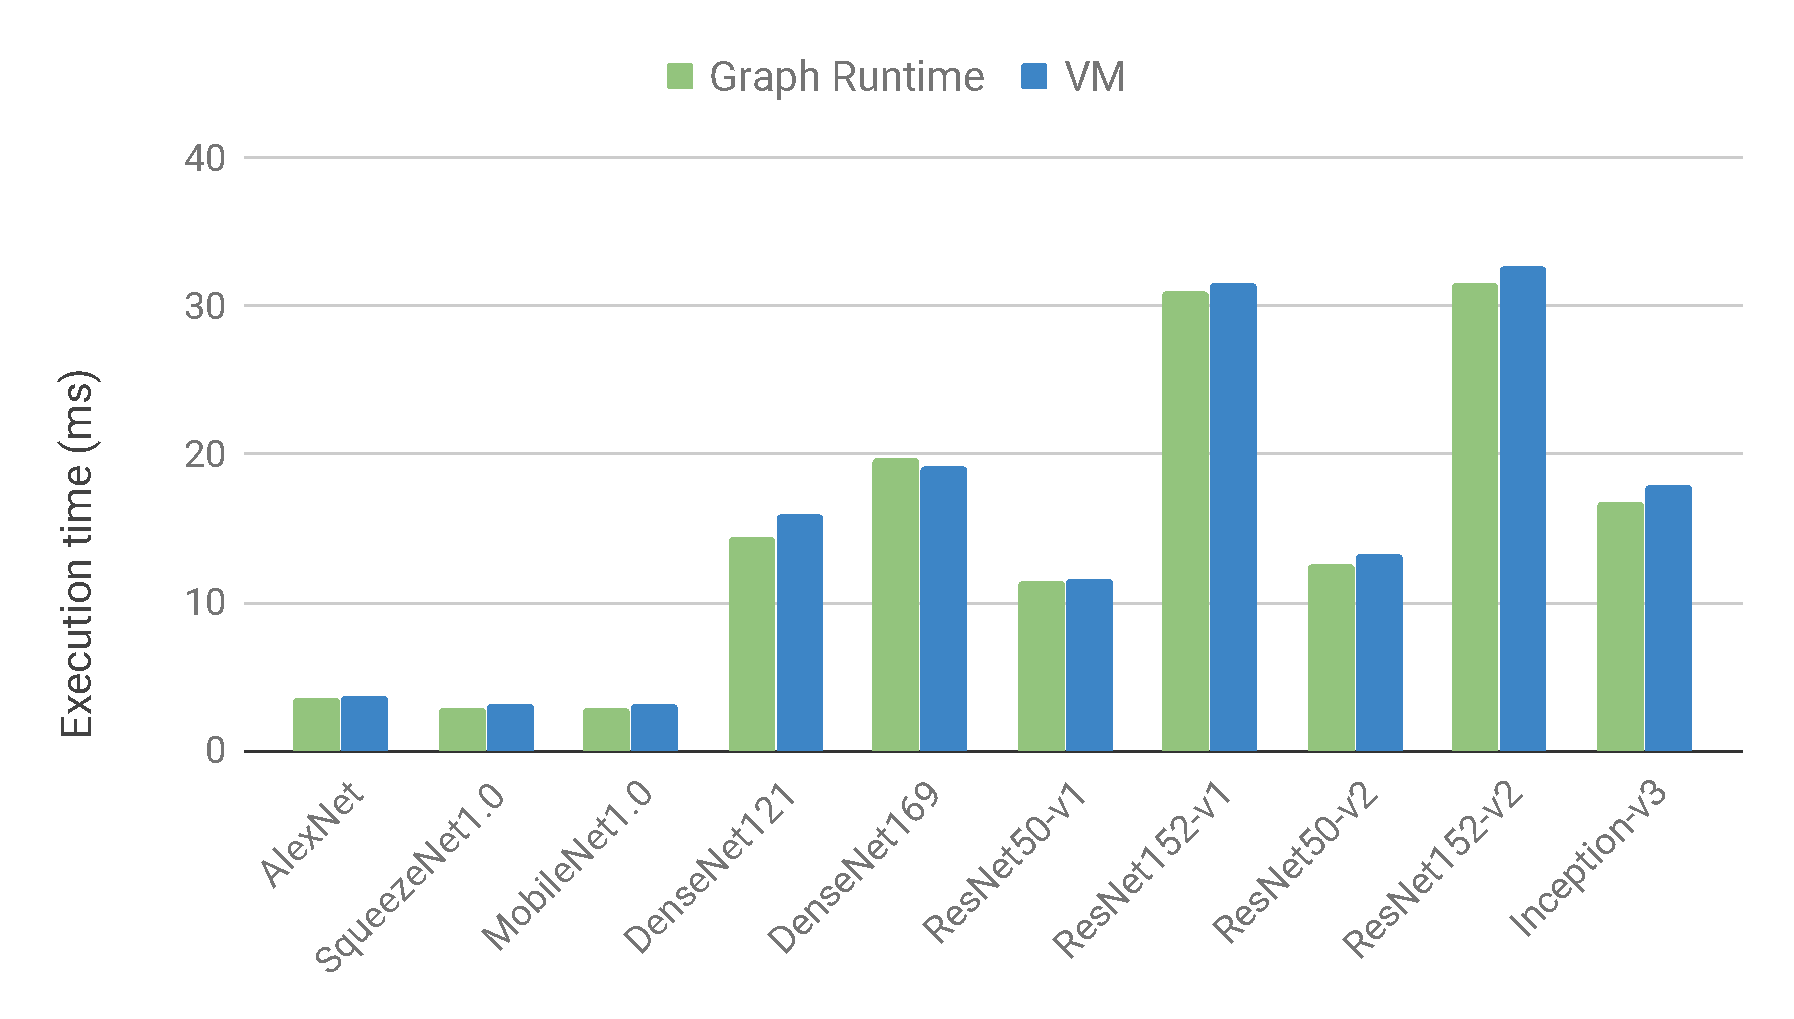
\includegraphics[width=.8\linewidth]{figs/cv_models.pdf}
  \caption{Benchmarking results of graph runtime vs. Relay.}
  \label{fig:benchmark}
\end{figure*}

\begin{table*}[t]
\centering
\begin{tabular}{llllrrc}
\toprule
\multicolumn{1}{c}{\multirow{2}{*}{input size}} & \multicolumn{1}{c}{\multirow{2}{*}{hidden size}} & \multicolumn{1}{c}{\multirow{2}{*}{\# layers}} & \multicolumn{1}{c}{\multirow{2}{*}{seq length}} & \multicolumn{2}{c}{latency (ms)}                         & \multicolumn{1}{c}{\multirow{2}{*}{speedup ($\times$)}} \\
\multicolumn{1}{c}{}                            & \multicolumn{1}{c}{}                             & \multicolumn{1}{c}{}                          & \multicolumn{1}{c}{}                            & \multicolumn{1}{c}{MxNet} & \multicolumn{1}{c}{Relay VM} & \multicolumn{1}{c}{}                             \\
\midrule
100                                             & 100                                              & 1                                             & 1                                               & 0.53                      & 0.03                         & 18.4                                             \\
100                                             & 100                                              & 1                                             & 20                                              & 4.74                      & 0.52                         & 9.2                                              \\
100                                             & 100                                              & 1                                             & 100                                             & 21.75                     & 2.57                        & 8.5                                              \\
100                                             & 100                                              & 2                                             & 100                                             & 30.53                     & 4.79                         & 6.4                                              \\
100                                             & 100                                              & 3                                             & 100                                             & 55.47                     & 7.04                         & 7.9                                              \\
200                                             & 600                                              & 3                                             & 100                                             & 67.14                     & 35.16                        & 1.9                                              \\
400                                             & 1150                                             & 3                                             & 100                                             & 166.54                    & 123.54                       & 1.3                                              \\
1500                                            & 1500                                             & 2                                             & 100                                             & 182.71                    & 138.78                       & 1.3
\\\bottomrule
\end{tabular}
\vspace{6pt}
\caption{Compare performance of LSTM models between MxNet and Relay VM.}
\label{tab:lstm}
\end{table*}

We evaluated the model inference with the VM against the TVM graph runtime on a number of popular vision models, including AlexNet, ResNet, MobileNet, VGG, DenseNet, SqueezeNet and Inception. Models are from GluonCV model zoo.  We repeated the inference 100 times for each model, obtained the performance result by averaging the execution times. All experiments were performed on Amazon EC2 C5.9xlarge instance (Intel Skylake-SP, 72 GiB memory, 18 physical cores, featured with AVX-512). In general, VM reached comparable inference performance even some optimizations were not plugged. As shown in \autoref{fig:benchmark}, we observed VM provided 2.59\% performance improvement on DenseNet169. On the rest of models, VM introduced some performance regression. We saw 11.3\% performance drop on SqueezeNet1.0.

We also evaluated the inference performance of recurrent models, which requires control flow support. We choose LSTM model \citep{hochreiter1997long} and vary the input size, hidden size, number of layers, and sequence length. We measured the execution time of LSTM models for both MxNet MKL 1.4.1 and Relay VM on Amazon EC2 C5.9xlarge instance. \autoref{tab:lstm} shows that Relay VM can achieve 6.4-18.4$\times$ speedup on small LSTM models and 1.3-1.9$\times$ speedup on larger models.
\end{comment}
